\documentclass[11pt]{report}

\usepackage[french]{babel}
\usepackage[utf8]{inputenc}

\usepackage[T1]{fontenc}

\usepackage{tipa}
\usepackage{tipx}

\usepackage{listings}

\title{
\includegraphics[scale=1]{logo.jpg}\\ \textbf{Rapport Finale De Projet Technologique}\\ Traduction de langage SMS\\ 1\up{ère} année}
\author{Réalisé par :\\
		Benjamin Fraquet\\
		Francisco Ruivo\\
		Maël Naccache\\
		Merouane Bousbaa\\\\
		Encadré par :\\
		Nicolas Hernandez}
		
\date{15/05/2013}

\usepackage{graphicx}
\begin{document}

\maketitle

\tableofcontents

\newpage

\begin{center}
\textbf{Résumé}
\newline
Ce projet consiste à transcire du langage "SMS" vers une phrase française compréhensible.
Ceci à été réalisé au moyen du language Prolog et de deux approches de traductions : Par dictionnaire et à l'aide de la phonétique.
Le rapport est divisé en deux grandes partie : Le chapitre 2 qui s'interesse à l'approche théorique du problème et le chapitre 3 qui explique la réalisation technique.
Le premier chapitre introduira rapidement le Prolog et le language SMS et la dernière partie expliquera l'utilisation du programme ainsi que les améliorations à apporter.
Sur ce, Bonne lecture.
\end{center}

\newpage

\chapter{Introduction}
	\section{Avant-Propos}
	Le sujet de notre projet technologique était la "Traduction de langage sms/chat/forum en francais". La seul contraintes était de réaliser le projet en Prolog via l'implémentation libre SWI-Prolog. Si vous vous posez la question de ce qu'est le langage SMS ou ce qu'est Prolog, téléporter vos yeux respectivement vers les sections 1.2 et 1.3. Ce qu'il faut brièvement comprendre c'est qu'il nous étais demandé de traduire un ensemble d'abréviation française vers une phrase compréhensible pour le commun des mortels. Nous devions donc créer une petite intelligence artificiel capable de faire ceci pour nous. Pour cela, plusieurs idée nous sont venu à l'esprit, elle seront aborder dans la section 1.4.
	\paragraph{} Sur ses mots, je vais vous laissez à l'immense joie de consulter le reste de ce rapport afin de découvrir le magnifique univers de la traduction, vu par des premières années. Une expérience qui je n'en doute point, ne manquera pas de vous surprendre ( en bien ou en mal, je ne garanti rien ).
	
	\section{Du langage SMS}
	Vous l'avez déjà sûrement rencontré, que ce soit par vos enfant, vos neveux, voire peut être même, vos étudiants, il y à peut de chance que vous y ayez échappé. Prenant la forme de message court et rarement compréhensible pour le non-initié, le langage SMS à pour origine, comme son nom l'indique, le SMS.
	\paragraph{}
	SMS est l'abréviation de {\em Short Message Service}\footnote{Source: wikipedia.org/wiki/Short\_Message\_Service} ( Comme l'on dirais en Anglais de spécialité ). Il fait partie de la norme GSM et fut développé dans les années 1980, toutefois, son ouverture au grand publique date des années 2000. Historiquement, pour des raisons techniques, la taille d'un SMS à du être limité à 128 octets, c'est à dire, environ 146 caractère ASCII 7bits. Il faut de plus noter que les forfaits proposant des SMS illimités par les opérateurs grands publique est relativement récente ( on commence à en voir apparaître en 2004 mais ceux-ci sont souvent limité au réseau de l'opérateur et coûteux\footnote{Exemple du premier forfait "Illimité" de Bouygue Telecom : lesmobiles.com/actualite/1453-bouygues-lance-le-premier-forfait-sms-illimite.html} ). Aussi, l'utilisation d'abréviation dans les SMS s'est démocratisé afin de pouvoir transmettre un maximum d'information à un minimum de coût.\\
	De plus, un autre facteur c'est rajouté à ceci : l'agencement E.161 utilisé dans la plupart des téléphones portables. En effet, il était relativement difficile d'embarqué un clavier classique à 102 touches tout en restant portable. Toutefois, cette agencement a plusieurs défaut : Il rend l'écriture plus longue, rend difficile d'accès les caractères accentués et spéciaux ( tel que l'apostrophe ) ainsi que les majuscules. Cela à pour conséquence une utilisation à outrance des abréviations, la suppressions des accents et tout autre caractères spéciaux ( qui de plus était bien souvent codé sur 1 octets ou plus au lieux de 7 bits, ce qui limitais d'autant plus la taille du SMS ) et utilisation de toute autre méthode pouvant réduire le temps de frappe et la taille du message.\\
	Le langage SMS était née.\\
	Malgré l'invention d'aide à la frappe ( tel que le T9\footnote{wikipedia.org/wiki/Text\_on\_9\_keys\#T9} ) et la généralisation des forfaits dit "illimités", le langage SMS continue toujours à être utilisé, notamment sur internet, puisqu'il permet de communiquer un message écrit en un minimum de temps et d'effort, au détriment de la qualité du dit message et du respect du récepteur qui aura bien souvent du mal à déchiffrer le message.\\
	Voici un exemple\footnote{Merci à Mr. Batiste Martin du Groupe 4 qui m'aura fournit cet exemple.} : \\
	\indent {\em slt comen sa va t ou y fo kon se voa}\\
	Que l'on traduirait :\\
	\indent {\em Salut. Comment ça va ? Tu est ou ? Il faut que l'on ce voit.}\\\\
	Vous serez vous même juge de la compréhensibilité de ce message.\\
	Nous allons désormais voir un autre langage, plus vieux que le SMS et surtout, plus formel.
	
	\section{De Prolog}
	Prolog, pour PROgrammation LOGique, fut conçu en 1972 par Alain Colmerauer et Philippe Roussel à l'Université d'Aix-Marseille. Bien que l'on trouve des langages utilisant principalement la logique plus ancien que Prolog ( Absys ou Planner en 1969 ), Prolog est le premier langage à réellement utilisé le paradigme de programmation logique.\\
	Prolog est un langage interprété, toutefois, il fonctionne différemment de ce que l'on voit chez Python, PHP, et autre langage interprété. En effet, en Prolog, l'interpréteur n'est pas la pour exécuter un programme, il est la pour apprendre et pour répondre à des questions. En effet, lorsque l'on code en Prolog on va en vérité créer des faits et des règles qui seront vrais si elle peuvent s'unifier et fausse sinon et on va les apprendre à notre interpréteur, on lui posera ensuite des questions et l'interpréteur nous répondra si elle sont vrais ou fausse en fonction de ce qu'on lui à appris. Il peut même, grâce au mécanisme d'unification, chercher pour une question, toute les réponses vrais.\\
	Il est compliquer de comprendre comment on peut programmer ainsi, toutefois, tout serra expliquer dans le Chapitre 3 et la section 4.1.
	
	\section{Avant de programmer, des idées !}
	Si vous ne le saviez déjà pas, vous devriez avoir désormais une vague idée de ce qu'est le langage SMS et le Prolog. Bien. Mais revenons au cœur du sujet : Comment allons nous traduire du SMS vers un français plus ou moins correcte ?
	\paragraph{}
	Deux grandes idées nous sont venu en tête. La première est relativement simple, il suffit de créer un dictionnaire de correspondance à la manière d'un dictionnaire français-anglais, par exemple. Il nous suffirais d'apprendre à notre petite intelligence artificielle la signification de chaque acronyme SMS pour qu'elle puisse traduire une phrase mot-à-mot.\\
	La seconde idée est de ce basé sur la phonétique des mots. En effet, en SMS certain mot change de forme mais pas de prononciation par exemple {\em Comment} peut s'écrire {\em komen} mais s'entendra toujours /\textipa{k\!Om\~a}/, on peut ainsi "deviner" la signification de certain mot.
	\paragraph{}
	Nous allons étudier ces idées plus en détails dans le chapitre qui suis.

\chapter{Partie Théorique}
	\section{Posons quelques Axiomes}
	Avant d'expliquer notre démarche il nous faut poser quelque axiomes que nous utiliserons dans notre traduction et expliquer pourquoi nous avons fait ces choix d'axiomes.\\
	Les voici : \\
	\begin{itemize}
		\item \textbf{1 - Le SMS ne change pas l'ordre des mots et de la ponctuation dans la phrase.}\\
		Le langage SMS n'est qu'un ensemble d'abréviation, aussi, il n'est pas sensé pouvoir changer la position d'un mot dans une phrase. Nous somme d'accord que {\em J'aime les patates.} et {\em J'patates. les aime} non pas la même signification, aussi {\em jm lé patat} et {\em jpatat lé m} sont tout autant différent.\\
		
		\item \textbf{2 - La traduction peut être ambigu}\\
		La traduction n'est pas une fonction, par la nous voulons dire qu'une même abréviation peut être traduite en plusieurs mot différent. Un exemple simple sont les conjugaison : {\em komenc} pourrait ce traduire {\em commencer}, {\em commencé} ou encore {\em commencez}.\\
		
		\item \textbf{3 - Un mot en SMS peut être traduit par un groupe de mot}\\
		Par exemple, {\em c.à.d} veut dire {\em C'est à dire}.\\
		
		\item \textbf{4 - Un mot est encadré par deux espaces}\\
		Ces cette définition d'un mot que nous choisissons pour notre traduction. Elle vous aura sûrement choqué au plus profond de votre petit cœur sensible. En effet, {\em J'étais} est constitué de deux mots, ors, selon notre définition, {\em J'étais} n'est qu'un mot. Alors, pourquoi cette hérésie ? Si vous avez bien lu la section 1.2, vous avez peut être déjà une petite idée. Rappelez-vous, nous avons parler de l'agencement E.161 qui rendais difficile d'accès les caractères spéciaux dont l'apostrophe et tout autre ponctuations fait partie. Aussi, il est relativement sur d'assumé d'une phrase SMS ne contiendra n'y apostrophe, ni ponctuation autre que des points d'exclamation ou d'interrogation ( en vérité, il s'agit plus souvent de $ \forall n \in [5;+\infty] | n \times ? \vee n \times ! $ ). Toutefois, nous allons tout de même traiter la ponctuation comme des mots, seul les apostrophes ne seront pas traité.\\
		\item \textbf{5 - Une phrase en SMS est entièrement en minuscule}\\
		Cette axiome est nécessaire du à un détail technique que nous expliquerons dans le Chapitre 3. Il peut ce justifier pour les mêmes raisons que l'axiome ci-dessus.\\
	\end{itemize}
	
	Nous voila désormais armé pour entamer nos traduction !
	
	\section{Larousse mon amour}
	Nous allons donc mettre en œuvre une traduction par dictionnaire. L'avantage de ce type de traduction est ça simplicité de mise en œuvre, sa rapidité et, dans le cas de langage que l'on peut traduire littéralement Mot-à-Mot comme le SMS, sa traduction quasi-parfaite si il n'y à pas d'ambiguïté. Pour cela, il nos faut juste créer une "base de connaissance" ( on peut voir ça comme une base de donnée relationnel ) m'étant en relation pour chaque abréviation SMS, le ou les mots français lui correspondant. Une fois que notre intelligence artificielle à pris connaissance de cette base, il lui suffit de "découper" une phrase mot à mot, selon l'axiome 4, et de traduire chacun d'entre eux grâce à sa base de connaissance.
	\paragraph{}
	Cette méthode à toutefois de gros défaut : Elle ne peut traduire un mot si il n'est pas dans ça base de connaissance, ne peut déterminer la traduction la plus probable dans le cas d'ambiguïté et nécessite de créer une énorme base de connaissance qui va devoir régulièrement changer. De plus, elle est incapable de s'adapter à des mots polymorphes en dehors de connaître leurs très nombreuses itération.\\
	En bref, on ne peut ce contenter de cette méthode et il nous faut trouver un autre moyen de traduction.
	
	\section{Super-phonétique à la rescousse !}
	Nous l'avons déjà aborder dans la section 1.4, nous pouvons utilisé la phonétique des mots pour les traduire.
	La mise en œuvre de cette méthode est légèrement plus compliquer : Elle nécessite de connaître tout les phonèmes de la langue française et de savoir découper un mot en tout ses phonèmes. Toutefois, une fois cette étapes faite, le reste s'avère relativement simple : Une fois le mot SMS traduit en son équivalent phonétique on va rechercher si on peut l'unifier avec un mot français lui même traduit en phonétique, si oui, alors il s'agit très probablement de ça traduction.
	\paragraph{} Noté comment j'ai précisé "probablement" dans la phrase précédente ? Et bien oui, la méthode par la phonétique n'est malheureusement pas parfaite. Si elle à l'avantage de traduire sans problèmes les mots polymorphes ( pour elle {\em komen}, {\em comen}, {\em coman}, etc ... sont pareilles ), il n'est pas garanti qu'elle fournisse une bonne traduction ( un mot en SMS peut avoir la même phonétique qu'un mot français sans être ce mot ) et, de plus, un simple modification d'en la phonétique entre l'abréviation et sa traduction réel, bien que négligeable par l'oreille humaine ( par exemple /\textipa{\~a}/ et /\textipa{\~O}/ sont relativement similaire ) fera rater la traduction par cette méthode.\\
	Nous avons donc opter pour une solution prenants en compte les avantages et défaut de chaque méthode.
	
	\section{Passons le tout au mixeur}
	Nous avons donc décidé d'utiliser des deux méthodes dans un ordres bien définie. Tout d'abords, on essaye de traduire la phrase via l'approche par dictionnaire et ensuite on utilise l'approche phonétique pour tout les mots que nous n'avons pu traduire précédemment. Faire ainsi à l'avantage de permettre de garder une base de connaissance relativement réduite, mais sure, pour l'approche par dictionnaire, permettant donc une traduction relativement fidèle, et de garder les mots variants pour l'approche par phonétique qui est plus adapté.\\
	Cette méthode n'est bien sur pas non plus exempt de défaut, toutefois, nous aborderons ceci dans la section 4.3 dans laquelle nous aborderons aussi les solutions techniques et théoriques à tout les problèmes que nous avons pu rencontrer.

\chapter{Partie Technique}
Cette partie va ce concentrer sur l'implémentation des idées proposés dans le Chapitre 2. Il présentera aussi le diffèrent problème technique rencontré lors de la réalisation du projet.

	\section{Un peu de dictionnaire dans mon Prolog}
	Avant d'essayer d'implémenter un dictionnaire en Prolog, essayons de modéliser ce que représente un dictionnaire.\\
	Nous pouvons voir un dictionnaire Français-SMS comme un ensemble de relation entre différents éléments ( ici, les mots ). Très simplement nous pouvons écrire ceci comme :\\
	\smallskip
	
		$ 
			Dictionnaire \in \{ \\
			\indent	"bjr" \rightarrow "bonjour"\\
			\indent "slt" \rightarrow "salut"\\
			\indent \}
		$\\
	
	\noindent Cette association d'élèment ce retrouve dans la plupart des langages sous la forme des tables de hachages. Toutefois, Prolog ne dispose pas de ce type de donnée, mais, du à la nature logique du langage, il est aisé de créer ce type de relation.\\
	Nous avons donc choisi d'utiliser les \emph{Fait} pour implémenter ceci. Un dictionnaire peut s'exprimer sous la forme d'un fait d'arité 2 comprenant un mot SMS et sont équivalent Français. L'équivalent de l'écriture relationnel précédent s'écrit donc en Prolog :\\
	
	\begin{lstlisting}[language=Prolog]
	dico('bjr','bonjour').
	dico('slt','salut').
	\end{lstlisting}
	
	Nous avons donc créer une première base de connaissance pour notre intelligence artificielle. Ainsi, nous pouvons déjà commencé à traduire grâce à l’interpréteur Prolog, par exemple, pour traduire {\em "bjr"} :
	\begin{lstlisting}[language=Prolog]
	?- dico('bjr',E).
	E = 'bonjour'.
	
	true.
	\end{lstlisting}
	
	Nous avons donc une première traduction par dictionnaire fonctionnel, toutefois celle-ci n'est pas très pratique à utiliser et ne traduit qu'un mot à la fois. Comment allons nous faire pour traduire des phrases ?\\
	Pour cela nous allons utiliser une {\em Règles}. Sans faire un cours de Prolog ( ce qui n'est pas le but de ce rapport et qui est hors de mes compétences ), une règles est simplement un terme complexe composé d'autre règle et de fait que l’interpréteur Prolog va chercher à unifier.
	\paragraph{}
	Nous pouvons donc écrire une règle récursive qui va parcourir une liste de mot en SMS en séparant la tête de la liste et la queue de la liste, va appliquer le fait {\em dico/2} sur la tête, placer le résultat dans la tête de la liste en second argument puis passer les queues des deux listes à elle même pour ainsi traduire toute la liste jusqu'à la fin :
	
	\begin{lstlisting}[language=Prolog]
	smsVersFr([],[]). % Cas final.
	smsVersFr([Tete|Queue],[Tres|Qres]) :-
		dico(Tete,Tres),  
		smsVersFr(Queue,Qres).
	\end{lstlisting}
	
	Cette règles nous permet donc de traduire une liste d'atomes ( Ici représentant des mots en SMS ) littéralement mot-à-mot. Par exemple :
	
	\begin{lstlisting}[language=Prolog]
	?- smsVersFr(['slt','bjr'],E). 
	E = [salut, bonjour].
	
	true.
	\end{lstlisting}
	
	Nous pouvons encore améliorer ce système en créant une règle prenant une chaîne de caractère et renvoyant les traductions trouvé. Pour cela, il nous suffit de découper la chaîne en liste d'atomes. Il existe une règles de SWI-Prolog permettant ceci, il s'agit de {\em atomic\_list\_concat/3}. Cette règles à trois argument : Une liste d'atomes, une chaîne qui servira de séparateur et la chaîne à découper. Nous utilisons un espace comme séparateur. Ce choix est du à l'Axiome 4, ce qui simplifie le système mais a pour principal défaut de ne pas gérer la ponctuation, par exemple, si l'on cherche à découper la phrase {\em "bjr, slt"} nous obtiendrons les atomes {\em ['bjr,', 'slt']}. {\em 'bjr,'} sera donc consiéré comme un mot, hors, notre dictionnaire connais {\em "bjr"} mais pas {\em "bjr\textbf{,}"}, cela empêchera donc la traduction. Nous expliquerons plus tard comment nous avons résolu ce problème. Pour le moment nous devons faire avec.\\
	La règles de découpage est donc simple à écrire :
	
	\begin{lstlisting}[language=Prolog]
	chaineVersAtom(Chaine, ListeAtom) :-
		atomic_list_concat(ListeAtom, ' ', Chaine).
	\end{lstlisting}
	
	Par exemple :
	
	\begin{lstlisting}[language=Prolog]
	?- chaineVersAtom('bjr slt', B).
	B = [bjr, slt].
	
	true.
	\end{lstlisting}
	
	Il nous suffit ensuite de créer une règles utilisant les règles précédentes pour traduire une chaine de caractère :
	
	\begin{lstlisting}[language=Prolog]
	traduire(Sms, Fr) :-
		chaineVersAtom(Sms, Liste),
		smsVersFr(Liste, Fr).
	\end{lstlisting}
	
	Ce qui nous donnera :
	
	\begin{lstlisting}[language=Prolog]
	?- traduire('bjr slt',E).
	E = ['bonjour', 'salut'].
	
	true.
	\end{lstlisting}
	
	Nous avons donc une traduction par dictionnaire fonctionnelle et simple d'utilisation. Une seul chose reste à régler : Que ce passe t'il si nous donnons à notre intelligence artificielle un mot qui n'est pas dans ça base de connaisance ?
	
	\begin{lstlisting}[language=Prolog]
	?- traduire('bjr lol',E).
	false.
	\end{lstlisting}
	
	{\em "lol"} n'étant pas dans ça base de connaissance, il ne peut unifier {\em dico('lol',X).} et répond donc que la requête est fausse.\\
	Nous pouvons forcer l'intelligence artificielle à traduire quand bien même elle ne connais pas le mot simplement en utilisant le fait {\em dico(X,X).}. Ce fait associera tout mot à lui même. Il doit être déclaré après toute les autres occurrences de dictionnaire ( autrement tout mot sera remplacer par ... lui même, ce qui n'est pas très intéressant ). En ajoutant ce fait on obtient donc :
	
	\begin{lstlisting}[language=Prolog]
	?- traduire('bjr lol',E).
	E = ['bonjour','lol'].
	
	true.
	\end{lstlisting}
	
	Ce comportement n'est pas forcément désirable puisque la traduction est de ce fait faussé mais cela permet à l'IA de fonctionner malgré tout.
	La traduction par dictionnaire est donc utilisable, la plus grande difficulté ici étant de créer une base de fait suffisamment grande pour traduire le plus de termes possibles.\\
	Toutefois, nous avons encore le problème d'être incapable de traduire les mots inconnus, pour cela nous avons développer une deuxième traduction.
	
	\section{Une /so.ly.sj\textipa{\~O}/ différente}
	Quel est le point commun{\em Comment}, {\em Komen} et {\em coman} ?\\
	Il ce prononce de la même manière ! En effet, les 3 ce traduise /\textipa{kOm\~a}/ en phonétique. Si nous arrivions à traduire les mot en SMS en phonétique, nous pourrions les comparés à une base connu de mot et ainsi trouver les traductions possibles du mot.\\
	Nous allons tout d'abord nous intéresser à la traduction d'un mot en SMS. Pour cela nous nous basons sur le système API Français pour avoir la liste des phonèmes\footnote{Source : https://en.wikipedia.org/wiki/Help:IPA\_for\_French}. Il nous faut donc créer une base de connaissance contenant ces phonèmes. Pour cela nous avons utilisé un script Ruby pour parser la syntaxe de la page wikipedia, les fichiers ruby et les regexp utilisé sont disponible dans la le dossier v2.0/ à la racine du projet.
	Nous avons donc créer un ensemble de fait dont voici certain exemple :\\
	
	\indent phon([99,104],'\textipa{k}').\\
	\indent phon([114],'\textipa{K}').\\
	\indent phon([114,104],'\textipa{K}').\\
	\indent phon([99,104],'\textipa{\:l}').\\
	\indent phon([115,99,104],'\textipa{\:l}').\\
	
	Vous vous demandez peut être ce que représente la liste en premier argument. En vérité, j'ai légèrement ( mais vraiment légèrement, et puis c'était pour votre bien d'abord ) menti qu'en je vous est présenté {\em 'slt bjr'.} comme étant une chaine. En vérité, en Prolog, toute chaîne écrite entre apostrophe est un atome. Une chaîne est en réalité une liste de nombre représentant le caractère en UTF-8 \& ASCII 7bits en base 10. Ici, puisque nous allons traiter les mots caractère par caractère il est important de traiter des vrais "Chaîne", auquel cas nous traiterions atomes par atomes, ce que nous ne souhaitons pas. Donc, cette base de connaissance pourrait ce lire :\\
	
	\indent phon('ch','\textipa{k}').\\
	\indent phon('r','\textipa{K}').\\
	\indent phon('rh','\textipa{K}').\\
	\indent phon('ch','\textipa{\:l}').\\
	\indent phon('sch','\textipa{\:l}').\\
	
	Bien, maintenant, comment convertir un mot en sont équivalent phonétique ? Tout d'abord il faut le convertir en chaîne. Cela ce fait via la règle name/2 de Prolog :
	
	\begin{lstlisting}[language=Prolog]
	?- name('Bonjour !',E). 
	E = [66, 111, 110, 106, 111, 117, 114, 32, 33].
	
	true.
	\end{lstlisting}
	
	Une fois ceci fait, il faut simplement convertir les caractères en phonèmes grâce au fait {\em phon/2} toutefois nous avons en problème. En effet, tout les phonèmes ne sont pas composé d'un même nombre de caractère, par exemple nous avons vu d'en notre base de connaisance que {\em r = \textipa{K}} ( 1 lettre = 1 phonème ) mais aussi que {\em rh = \textipa{K}} ( 2 lettres = 1 phonème ). Comment faire pour gérer cela ?\\
	Et bien cela est simple puisque les listes en Prolog sont {\em Magique}. Vous vous rappelez peut être de la notation {\em [T|Q]} que nous avons utilisé dans la traduction par dictionnaire pour obtenir la tête et la queue d'une liste ? Et bien il est tout a fait possible d'écrire {\em [T1,T2,...,Tn|Q]} pour récupérer n élément en tête de liste.\\
	Sachant que un phonème en français n'est pas composer de plus de 3 lettres, nous avons juste à dériver la règle de traduction en 3 variantes : une prenant 1 lettres, une en prenant 2 et une dernière en prenant 3.\\ 
	La règle est très similaire à la règle smsVersFr/2 vu dans la traduction par dictionnaire. Elle prend 2 listes en arguments, applique un fait sur la ou les têtes de la 1\up{ère} liste, la place dans la tête de la 2\up{ème} liste puis s'applique récursivement sur les queues des listes :
	
	\begin{lstlisting}[language=Prolog]
	getPhon([],[]).
	getPhon([T1,T2,T3|R],[H|Q]) :- phon([T1,T2,T3],H), getPhon(R,Q).
	getPhon([T1,T2|R],[H|Q]) :- phon([T1,T2], H), getPhon(R,Q).
	getPhon([T1|R],[H|Q]) :- phon([T1],H), getPhon(R,Q).
	\end{lstlisting}
	
	Ainsi, si nous essayons de traduire {\em Chat} en phonétique nous écrivons :
	\begin{lstlisting}[language=Prolog]
	?- name('chat',X), getPhon(X,B).
	\end{lstlisting}
	\indent \indent \indent \indent X = [99, 104, 97, 116],\\
	\indent \indent \indent B = [\textipa{\:l}, a, s] ;\\
	\indent \indent \indent X = [99, 104, 97, 116],\\
	\indent \indent \indent B = [\textipa{\:l}, a, t] ;\\
	\indent \indent \indent X = [99, 104, 97, 116],\\
	\indent \indent \indent B = [\textipa{\:l}, \textipa{A}, t].\\
	\begin{lstlisting}[language=Prolog]
	true.
	\end{lstlisting}
	
	Prolog va générer toute les traductions possibles grâce à ça base de connaissance. Nous pouvons noter qu'elle ne sont pas toute entièrement fidèle au mot toutefois, nous avons fait le choix de garder cette approximation car nous cherchons à traduire en phonétique du SMS, qui lui n'est pas forcément fidèle au mot d'origine non plus.\\
	Cette marge d'approximation permet ainsi d'augmenter les traductions possibles et donc la probabilités de générer une traduction que l'utilisateur jugera correcte.
	\paragraph{}
	Pour simplifier l'utilisation de cette règles on va créer une autre règle :\\
	enPhonetique/2 traduit un atome en phonétique :
	\begin{lstlisting}[language=Prolog]
	enPhonetique(Mot,Trad) :-
		atom_codes(Mot,Liste),
		getPhon(Liste,Trad).
	\end{lstlisting}
	
	Notons ici que {\em atom\_codes/2} est similaire à {\em name/2}. On obtient donc :
	\begin{lstlisting}[language=Prolog]
	?- enPhonetique('sha', B).
	\end{lstlisting}
	\indent \indent \indent \indent  B = [\textipa{\:l}, a] .
	\begin{lstlisting}[language=Prolog]
	true.
	\end{lstlisting}
	
	Bien, maintenant que nous pouvons traduire un mot SMS en phonétique, il serait pratique de s'en servir pour la traduction. Pour cela nous avons 2 choix : Utiliser une base de mot français et comparer les traductions phonétiques entre le mot SMS et la base, ou, utiliser une base de connaissance comprenant une base de mot en français et leurs phonétiques.\\
	Nous avons décider de prendre la deuxième solution. Ce choix c'est fait pour plusieurs raison :\\
	Tout d'abord, la première solution supposais d'essayer d'unifier chaque traduction phonétique possible de chaque mot français à chaque traduction phonétique possible du mot SMS ce qui aurais créer un nombre tellement important de combinaison qu'il aurait fallu Sequoia\footnote{https://fr.wikipedia.org/wiki/Sequoia\_\%28supercalculateur\%29} pour avoir une chance d'obtenir un jour des résultats.\\
	Ensuite, nous avons évoqué le fait que la traduction phonétique était approximative, de ce fait, la 1\up{ère} solution aurait créer de nombreux faux résultat conséquence d'approximation faite pour le mot SMS et Français.
	\paragraph{}
	La deuxième solution nécessite toutefois de trouver un dictionnaire Français-Phonétique. Pour cela, nous avons parsé un dump du wiktionary\footnote{wiktionary.org} mis à notre disposition par Mr. Hernandez ( notre professeur encadrant ).
	Nous avons pu ainsi générer une base de fait dont voici quelque exemple :\\
	
	\indent pron('lire','li\textipa{R}').\\
	\indent pron('nouveau','nuvo').\\
	\indent pron('mai','m\textipa{E}').\\
	
	Ensuite, nous avons créer une règle transformant une liste d'atome en chaîne :
	\begin{lstlisting}[language=Prolog]
	toString([],[]).
		toString([T|Q],[H|C]) :-
		atom_codes(T,H),
		toString(Q,C).
	\end{lstlisting}
	
	{\em atom\_codes/2 est similaire à name/2}\\
	
	Puis nous avons créé une règle qui traduit un mot SMS vers du Français grâce à la phonétique :
	\begin{lstlisting}[language=Prolog]
	traduirePhoneme(Mot,Trad) :-
		enPhonetique(Mot,Phon),
		toString(Phon, String),
		flatten(String, Liste),
		name(Ss,Liste),
		pron(Trad,Ss).
	\end{lstlisting}
	
	{\em flatten/2 sert à simplifier une liste composer. Par exemple [[42,13],25,65,[25]] devient [42,13,25,65,25].}\\
	
	Par exemple :
	\begin{lstlisting}[language=Prolog]
	?- traduirePhoneme('sha', B).
		B = chat ;
		B = chas ;
		B = chas ;
		B = chah ;
		B = schah ;
		B = 'Chat' ;
		B = 'Chat' .
		
	true.
	\end{lstlisting}
	
	Voila, nous avons une traduction phonétique fonctionnelle. Elle n'est pas parfaite, loin de la, aussi nous allons voir comment tirer profit du meilleur des deux traduction dans la prochaine partie.
	
	\section{But, will it blend ?}
	
	L'objectif est donc d'utiliser les deux types de traductions afin d'obtenir la meilleur traduction possible. Pour faire cela, il nous faut tout d'abord déterminer l'ordre des traductions. Nous avons décidé de priorisé la traduction par dictionnaire car celle-ci assure une traduction plus sur. De plus, la traduction par phonétique est parfaite pour déterminer des mots que l'on ne connaît pas, aussi cette ordre semble le plus efficace.\\
	Ceci décidé, créer une règle utilisant les deux traductions est extrêmement simple :
	\begin{lstlisting}[language=Prolog]
	traduireMot(Sms, Fr) :- dico(Sms, Fr).
	traduireMot(Sms, Fr) :- traduirePhoneme(Sms, Fr).
	traduireMot(Sms, Sms).
	\end{lstlisting}
	
	Cette règle va donc essayer de traduire un mot via la traduction par dictionnaire, puis, si elle échoue, elle va essayer de le traduire avec la phonétique et enfin, si les deux traductions échouent, alors on ne traduit simplement pas le mot. A la manière du fait {\em dico(X,X).} cela assure que la traduction est tout de même effectuer. À noter d'ailleurs que si l'on souhaite que {\em traduireMot/2} fonctionne, il faut supprimer {\em dico(X,X).} car sinon, {\em dico/2} sera toujours vrais ce qui faussera notre traduction.\\
	
	Ensuite, si nous désirons traduire simplement une "phrase" représenté par une liste d'atomes, il nous suffit de reprendre la règle {\em smsVersFr/2} et de la modifier pour utiliser la règle {\em traduireMot/2} :
	\begin{lstlisting}[language=Prolog]
	traduireMotaMot([],[]).
		traduireMotaMot([Tete|Queue], [Tres|Qres]) :-
		traduireMot(Tete,Tres), traduireMotaMot(Queue,Qres).
	\end{lstlisting}
	
	{\em Note : En utilisant traduireMot/2 ainsi, on essaye de respecter l'ordre des traductions, toutefois, du au fonctionnement de Prolog, il va essayer de générer toute les combinaisons possibles, autrement dit, il peut essayer de traduire une phrase entièrement grâce à la phonétique quand bien même dico/2 pourrait être vrais. Toutefois, les premières traductions respecterons l'ordre. Aussi, bien qu'il existe des méthodes pour éviter ce comportement ( notamment grâce à cut/1 ) nous avons décidé de le garder pour générer plus de traduction possible.}\\
	
	Sont utilisation est relativement simple et efficace :
	\begin{lstlisting}[language=Prolog]
	?- traduireMotaMot([slt, komen, va, ton, sha, ?],E).
		E = [salut, comment, vas, ton, chat, ?] ;
		E = [salut, comment, vas, ton, chas, ?] ;
		E = [salut, comment, vas, ton, chas, ?] ;
		E = [salut, comment, vas, ton, chah, ?] ;
		E = [salut, comment, vas, ton, schah, ?] ;
		E = [salut, comment, vas, ton, 'Chat', ?] ;
		E = [salut, comment, vas, ton, 'Chat', ?] ;
		E = [salut, comment, vas, ton, chats, ?] .
	\end{lstlisting}
	
	Pour encore plus de simplicité d'utilisation, on peut réutiliser la règle {\em chaineVersAtom/2} écrite plus tôt afin de prendre une pseudo-chaine plutôt qu'un tableau :
	\begin{lstlisting}[language=Prolog]
	traduire(Sms, Fr) :-
		chaineVersAtom(Sms, Trad),
		traduireMotaMot(Trad, Fr).
	\end{lstlisting}
	
	Ce qui nous donne :
	\begin{lstlisting}[language=Prolog]
	?- traduire('slt komen va ton sha ?',E).
		E = [salut, comment, vas, ton, chat, ?] .
	\end{lstlisting}
	
	Voila, nous avons une traduction fidèle et simple à utiliser. Nous pourrions nous arrêter la, toutefois, il nous reste quelques éléments à finaliser. 
	
	\section{Finissions}
	La première chose est, que ce passe t'il si l'utilisateur rentre des mots contenants des majuscules ?\\
	Nous avons vu que {\em "komen"} était correctement traduis. Voici ce qu'il ce passe si l'on essaye de traduire {\em "\textbf{K}omen"} :
	\begin{lstlisting}[language=Prolog]
	?- traduireMot('Komen', B).
		B = 'Komen'.
	\end{lstlisting}
	
	Nous aurions le même résultat si nous utilisions le dictionnaire avec {\em "s\textbf{L}t"}. Ceci vient du fait que pour Prolog, l'atomes {\em "a"} et {\em " 'A' "} ne sont pas les mêmes :
	\begin{lstlisting}[language=Prolog]
	?- a = 'A'.
	
	false.
	\end{lstlisting}
	
	{\em Note : Nous mettons "A" entre apostrophe car sinon, il serait considéré comme étant une variables et non pas un atomes.}\\
	
	Pour éviter ce genre de problème, nous pouvons simplement utiliser la règle de SWI-Prolog {\em downcase\_atom/2} qui va renvoyer la version en minuscule d'un atome :
	\begin{lstlisting}[language=Prolog]
	lowcase([],[]).
	lowcase([T1|R],[H|Q]) :- downcase_atom(T1,H), lowcase(R,Q).
	\end{lstlisting}
	
	Ce qui nous donne :
	\begin{lstlisting}[language=Prolog]
	?- lowcase(['Komen', 'sLt'], B), traduireMotaMot(B, X).
		B = [komen, slt],
		X = [comment, salut] .
	\end{lstlisting}
	
	C'est déjà une première chose de réglé. maintenant, que ce passe t'on si on utilise de la ponctuation ? Et bien essayons :
	\begin{lstlisting}[language=Prolog]
	?- traduire('bjr, komen',B).
		B = ['bjr,', comment] .
	\end{lstlisting}
	
	Il ne fait pas de distinction entre les caractères "normaux" et la ponctuation, et donc créer l'atome {\em "bjr\textbf{,}"} au lieux de {\em "bjr"} ce qui fait échoué la traduction.\\
	Pour traiter cela nous avons fait une petite règle simple : Le principe est de remplacer tout les caractère {\em "',;:.,?!} par leurs équivalent encadré de 2 espaces ( de manière à ce que {\em "bjr,"} soit traité mais aussi {\em ",bjr"} ). Par exemple {\em "komen."} va devenir {\em "komen<espace>.<espace>"}.\\
	Pour cela on créer un fait qui associe chaque caractère de ponctuation par sont équivalent encadré d'espace :
	\begin{lstlisting}[language=Prolog]
	ponc(44, [32,44,32]).
	ponc(46, [32,46,32]).
	ponc(63, [32,63,32]).
	ponc(33, [32,33,32]).
	ponc(58, [32,58,32]).
	ponc(59, [32,59,32]).
	ponc(E,E).
	\end{lstlisting}
	
	Puis on parcours un mot et on applique le fait sur les caractères parcourue :
	\begin{lstlisting}[language=Prolog]
	cleanup([],[]).
	cleanup([T|R], [H|Q]) :- ponc(T,H), cleanup(R,Q).
	\end{lstlisting}
	
	Finalement, on fait une règle qui va convertir un atome et renvoyer la chaine traiter :
	\begin{lstlisting}[language=Prolog]
	traiterPonctuation(Chaine, ChaineTraiter) :-
		name(Chaine, Liste), cleanup(Liste, ListeTraiter),
		flatten(ListeTraiter, Final), name(ChaineTraiter, Final).
	\end{lstlisting}
	
	Et on l'intègre à notre règle {\em chaineVersAtom/2} :
	\begin{lstlisting}[language=Prolog]
	chaineVersAtom(Chaine, ListeAtom) :-
		traiterPonctuation(Chaine, ChainePonc),
		atomic_list_concat(Atoms, ' ', ChainePonc),
		lowcase(Atoms, ListeAtom).
	\end{lstlisting}
	
	Et voila ! Notre traduction marche désormais quelque soit la ponctuation et la casse utilisé :
	\begin{lstlisting}[language=Prolog]
	?- traduire('Komen, va Ton sHa?',E).
	E = [comment, ',', '', vas, ton, chat, ?, ''] .
	\end{lstlisting}
	
	Comme finissions, nous pouvons même créer une règle un peu plus user-friendly en utilisant la règle {\em read/1} et {\em write/1} de SWI-Prolog :
	\begin{lstlisting}[language=Prolog]
	reduireFosse :-
		write('Veuillez ecrire la chaine a traduire :'),nl,
		read(X), traduire(X,Fr), write(Fr).
	\end{lstlisting}
	
	Ce qui nous donne :
	\begin{lstlisting}[language=Prolog]
	?- reduireFosse.
	Veuillez ecrire la chaine a traduire :
	|: 'komen va ton sha ?'.
	comment vas ton chat  ?  
	true ;
	comment vas ton chas  ?  
	true ;
	comment vas ton chas  ?  
	true .
	\end{lstlisting}
	
	Notre programme final ressemble donc a ceci :\\
	\begin{figure}[htp]
	\centering
	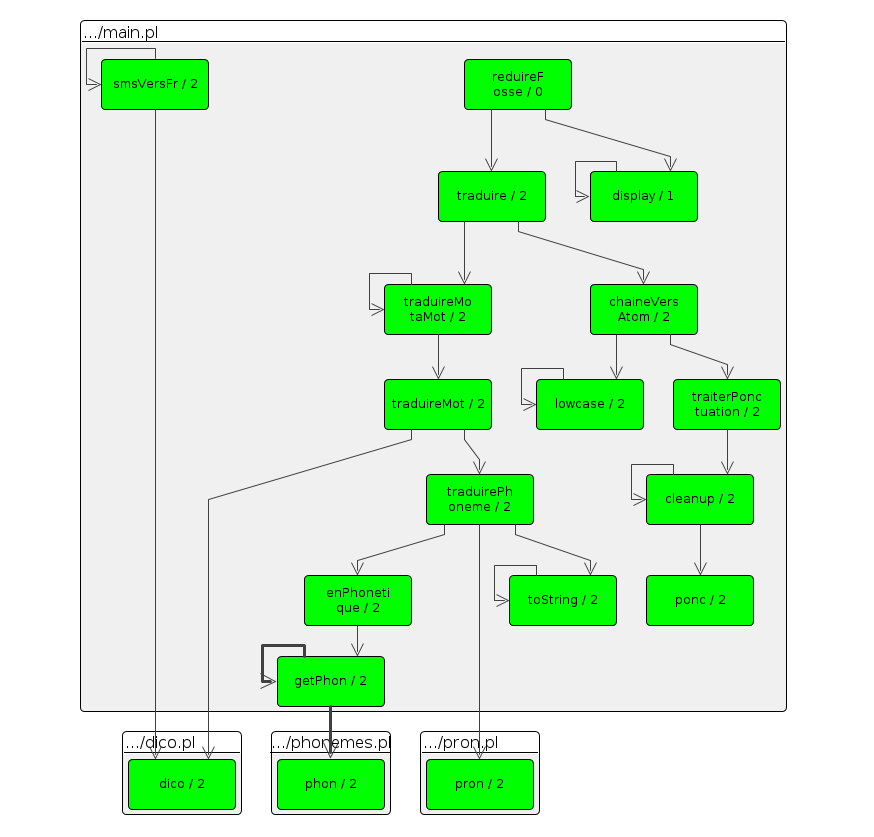
\includegraphics[scale=0.60]{mainpl.png}
	\caption{Graphique du programme. Les boites vertes représentes les règles et les faits, les flèches les appelles fait.}
	\end{figure}
 
\chapter{Conclusion}
	\section{A vous de jouer}
	Bien, vous savez désormais comment fonctionne la traduction, mais vous aimeriez surtout traduire le message mystérieux envoyer par votre neveux. Pour cela, il faut faut télécharger SWI-Prolog\footnote{http://www.swi-prolog.org/download/stable} puis ouvrir la console SWI-Prolog ( {\em swipl} sous GNU/Linux ) et consulter le fichier de projet. Pour cela écrivez juste {\em [/chemin/vers/le/fichier/main].} ( à noter qu'il ne faut pas rajouter l'extension de fichier {\em .pl} dans le chemin ). Le fichier main.pl s'occupera de charger tout les autres fichiers nécessaire. Une fois ceci fait, vous pouvez utiliser les règles {\em reduireFosse/0} et {\em traduire/2} comme vu précédemment.\\
	Voila ! A vous de jouer !
	
	\section{Les insectes attaques !}
	Aucun problème n'est parfait, le notre n’échappe pas non plus à quelque bug. Si l'utilisation de Prolog qui esy un langage haut niveau permet de ce soustraire des bugs techniques, il réside certain défaut :\\
	La traduction par phonétique est très dépendante de son dictionnaire, hors, du à l'irrégularité de la syntaxe Wikipedia, le fichier de dictionnaire à été grossièrement parsé et possède de nombreux bug ( par exemple, à un moment, {\em "sha"} était traduit {\em "phytotoxique"} car une erreur de parsage avait donnée à ce dernier la phonétique "\textipa{\:la}" ).\\
	De plus, notre algorithme de traduction vers la phonétique est souvent erroné du au fait que les phonèmes du français ne sont pas toujours exactement utiliser dans le SMS ce qui résulte en des erreurs de traduction.\\
	La traduction est donc encore loin d'être parfaite et nécessiterais encore des améliorations. 
	
	\section{Voyons plus grand ! Voyons plus loin !}
	Et bien, puisque nous parlions d'amélioration, voyons un peu celle que, si nous avion eu plus de temps, nous aurions pu apporter.\\
	Tout d'abord, pour améliorer la traduction, nous aurions pu utiliser un {\em modèle de langue}. C'est une méthode statistique qui permet de déterminer les régularités d'un langage. En d'autre terme, nous aurions pu déterminer la probabilité de la traduction d'un mot en fonction des mots qui l'entoure.\\
	Une autre amélioration qui n'est pas rapport à la traduction est celle de créer une GUI. SWI-Prolog permet d'embarquer son interpréteur dans de nombreux langage, dont Java. Nous aurions donc pu très bien imaginer créer une application Android\footnote{https://fr.wikipedia.org/wiki/Android} qui aurais permis à l'utilisateur de traduire simplement les SMS qu'il reçoit.
	
	\section{Credit}
	Avant de finir ce rapport, nous tenons à remercier plusieurs organisations et personnes pour l'aide, directe ou indirecte, qu'ils nous on apporté :
	\begin{itemize}
		\item Monsieur Nicolas Hernandez, notre professeur encadrant pour l'aide et les conseils qu'il nous à apporté.
		\item La fondation Wikimedia sans qui nous n'aurions pu obtenir simplement la liste des phonèmes Français et un dictionnaire phonétique. A ce titre, et au tire de la licence GFDL, tout crédit leurs reviens pour les fichiers phonemes.pl et pron.pl.
		\item Alain Colmerauer, Philippe Roussel et toute autre personne ayant participer à la conception de Prolog, sans quoi ce projet n'aurais jamais exister.
		\item Jan Wielemaker et tout les contributeur à SWI-Prolog pour avoir créer un interpréteur Prolog sous licence libre extrêmement puissant.
		\item  Patrick Blackburn, Johan Bos, et Kristina Striegnitz pour leurs cours sur Prolog {\em "Learn Prolog Now !}\footnote{http://www.learnprolognow.org/} qui nous aura aidé durant notre apprentissage de Prolog.
		\item Et finalement, Emmanuel Adam pour ses cours et exercices Prolog.
	\end{itemize}
	
	\newpage
	
	\begin{center}
		\Huge Rapport de Projet Technologique\\
		\bigskip 
		\bigskip 
		\bigskip 
		\bigskip 
		\LARGE Université de Nantes\\ Institut Universitaire de Technologie\\ Département Informatique
	\end{center}
	
\end{document}
